\section{Ejemplos de ejecución}
Se pueden encontrar encontrar multiples ejemplos de ejecución dentro del directorio \textit{ejemplos} en el repositorio. Veamos algunos:

Supongamos que tenemos 5 monedas:

\begin{lstlisting}
    [96, 594, 437, 674, 950]
\end{lstlisting}

En cada turno, Sophia tiene la opcion de elegir 2 monedas, la del principio o la del final. Esto implica que cada turno puede representarse como 2 opciones posibles, donde se debe elegir la opcion que acumule el mayor valor.

Para esto se recorren las opciones de manera recursiva, y se va seleccionando el maximo de los valores agregados en cada turno.

De esta forma, como se puede observar en el siguiente grafico, Sophia puede obtener un maximo de 1.483 puntos.

\begin{center}
    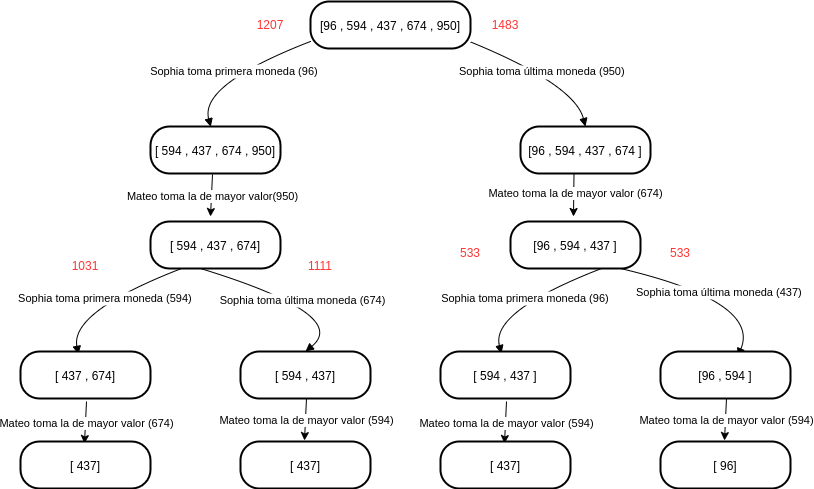
\includegraphics[scale = 0.5]{ {images/TDA-TP2.png} } 
\end{center}

Veamos lo que obtenemos al ejecutar en código el ejemplo que acabamos de ver:

\begin{center}
    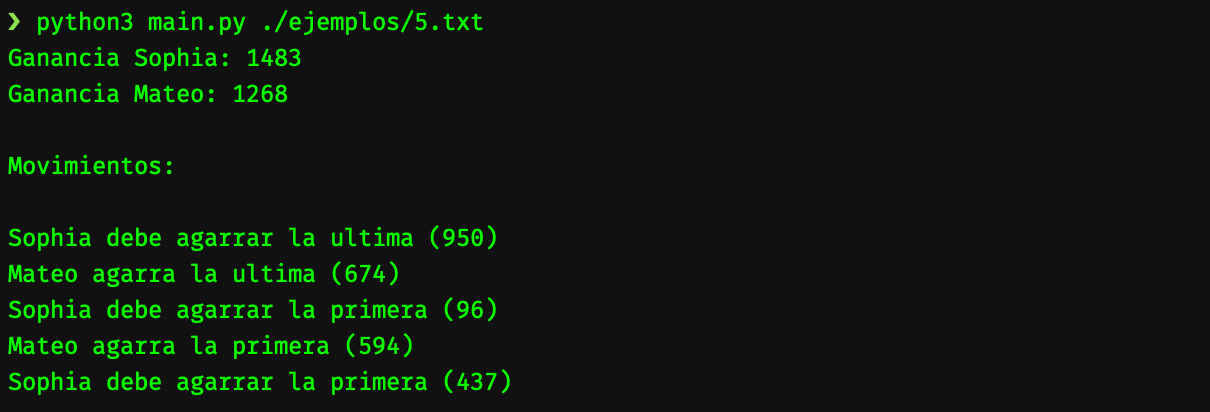
\includegraphics[scale = 0.6]{ {images/screen3.png} } 
\end{center}

Veamos la ejecución de otros ejemplos brindados por la cátedra:
\vskip0.5cm
Este ejemplo es con 10 monedas:
\begin{center}
    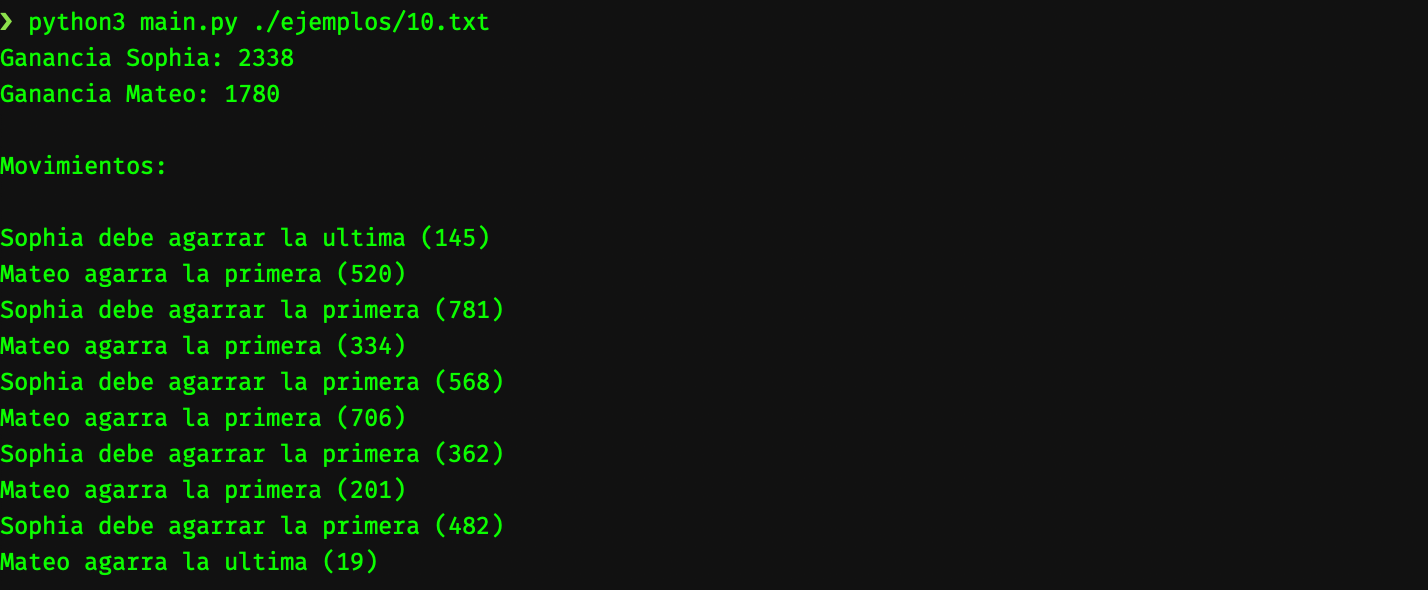
\includegraphics[scale = 0.6]{ {images/screen1.png} } 
\end{center}
Este ejemplo es con 25 monedas:
\begin{center}
    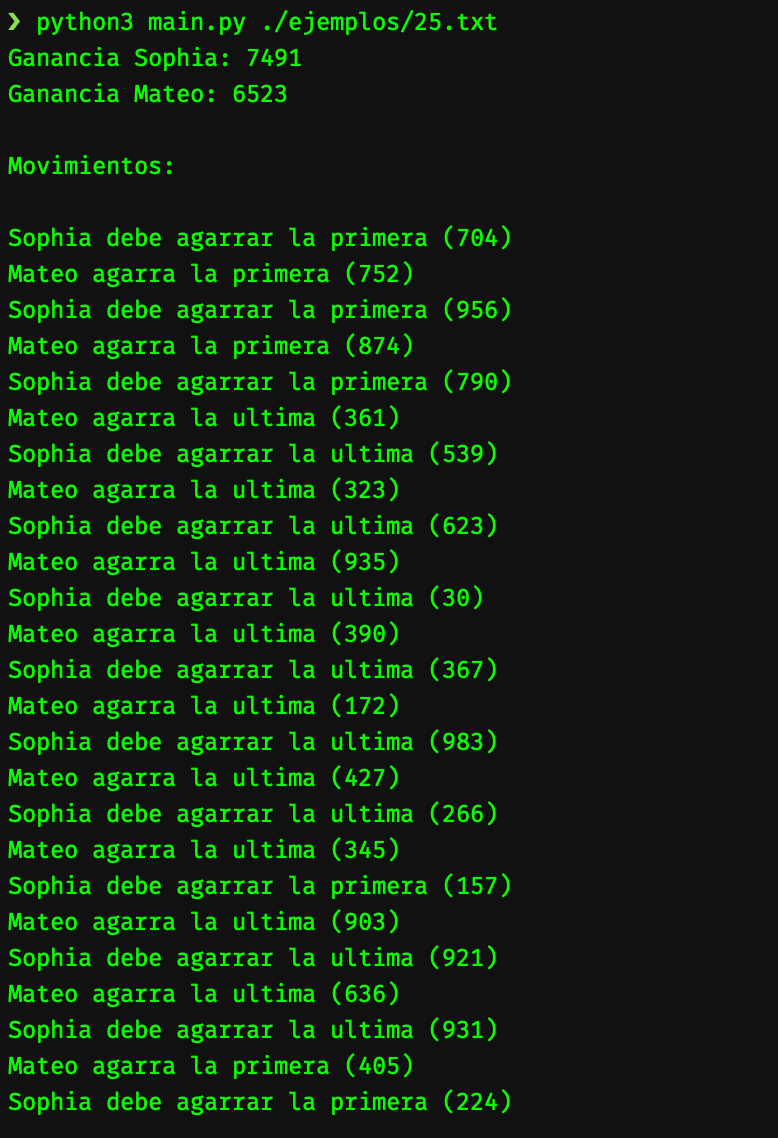
\includegraphics[scale = 0.6]{ {images/screen2.png} } 
\end{center}

Como podemos observar, los resultados obtenidos coinciden con los \textit{Resultados esperados} compartidos por la cátedra.

Ademas de estos ejemplos, se pueden encontrar otros en el directorio \textit{ejemplos} del repositorio. Los mismos pueden ser ejecutados con el comando \textit{pytest -v -s} en la terminal.

\begin{center}
    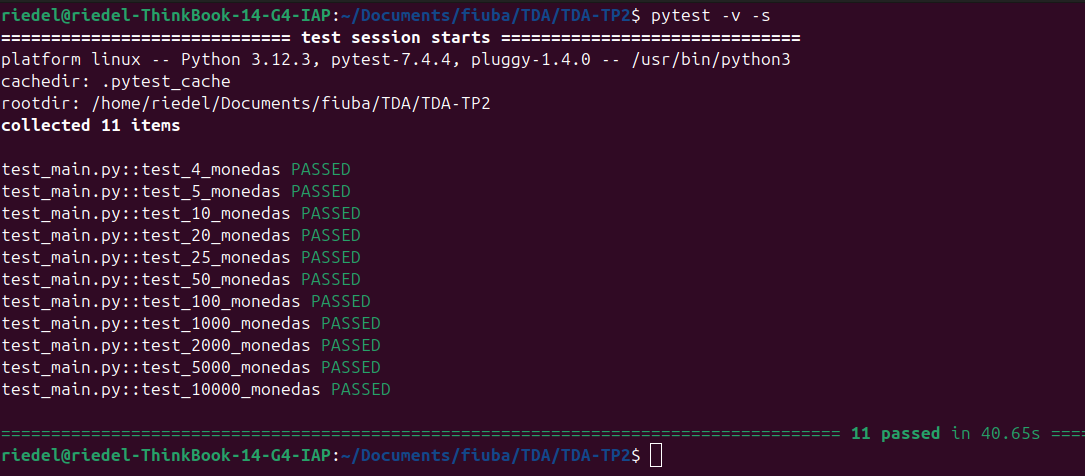
\includegraphics[scale = 0.4]{ {images/tests.png} } 
\end{center}